\section{Graph Algorithm}

\subsection{Basic Stuff}

\subsubsection{Fundamental Concept}
The following is the basic concept of graph.
\begin{enumerate}
    \item A \textbf{graph} is a pair $G = (V,E)$.
    \item $V$ is set of vertices or nodes.
    \item $E$ is set of edges. An edge $e$ in $E$ is a pair of
        vertices $e = \{u,v\}$.
    \item If $G$ is undirected, $e$ is unordered, i.e. $e = uv = vu$.\\
        If $G$ is directed, $e$ is ordered, i.e. $e = u \rightarrow v$ or $(u,v)$.
    \item Graphs represent relations between pairs of objects.
\end{enumerate}

In this course, we mainly consider simple graphs,
no multi-edges and no self-loop.

\subsubsection{Concepts Used in this Note}
The following conclude the terminology and notations used
in this notes.

\begin{enumerate}
    \item The \textbf{degree} of $v$ is the number of adjacent edges.
    \item $n$ denotes $|v|$, $m$ denotes $|E|$.
    \item For undirected graph: $\displaystyle m \leq \binom{n}{2}$.
        For directed graph: $\displaystyle m \leq 2 \binom{n}{2}$.
    \item Sub-graph of $G=(V,E)$ is a graph $G^\prime = (V^\prime, E^\prime)$,
        s.t. $V^\prime \subseteq V$, $E^\prime \subseteq E$.
    \item A \textbf{walk} is a sequence $v_1\ldots v_l$,
        s.t. $v_i \in V$ and $v_iv_{i+1} \in E$.
    \item A \textbf{path} is a walk where $v_i$ distinct.
    \item A walk is close, if $v_i = V_k$.
    \item A cycle is a ``closed path''.
    \item Undirected graph connected if path between every pair $u,v \in V$.
    \item If not connected, a component is a maximal connect sub-graph.
    \item A \textbf{tree} is a connected ``acyclic'' graph.
    \item A \textbf{forest} is a graph where each component is a tree.
    \item A \textbf{Spanning Tree} of $G$ is a sub-graph that is a tree
        and contains all vertices of $G$.
    \item For directed graps: directed path/cycles.
    \item A graph is \textbf{Strongly Connected} if directed path
        from any vertex to another exists.
    \item Directed acyclic graph is called a \textbf{DAG}.
\end{enumerate}

\subsubsection{Graph Data Structure}
There are two widely used data structure of graph:
\begin{itemize}
    \item Adjacency Matrix: $|V| \times |V|$ matrix, where $A[i,j] = 1$
        if $(i,j) \in E$.
    \item Adjacency List: an array of length $|V|$, where
        every entry in the array stores a list of neighbors.
\end{itemize}

For example:
\begin{figure}[ht!]
    \caption{Example Graph}\label{example_graph}
    \centering
    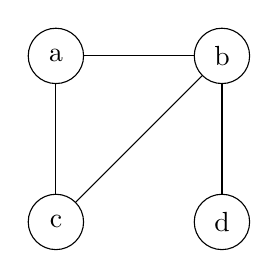
\begin{tikzpicture}
        \tikzstyle{every node}=[draw,circle,minimum size = 2em,node distance = 6em]
        \node (a) {a};
        \node [right of = a] (b) {b} edge(a);
        \node [below of = a] (c) {c} edge(a) edge(b);
        \node [below of = b] {d} edge(b);
    \end{tikzpicture}
\end{figure}

The adjacency matrix and adjacency list for \cref{example_graph} would be:
\begin{table}[ht!]
\begin{minipage}[b]{0.56\linewidth}
\centering
    \begin{tabular}{l|llll}
        & A & B & C & D \\ \hline
         A & 0  & 1  & 1  & 0  \\
         B & 1  & 0  & 1  & 1  \\
         C & 1  & 1  & 0  & 0  \\
         D & 0  & 1  & 0  & 0  \\
    \end{tabular}
    \caption{Adjacency Matrix}
    \label{table:student}
\end{minipage}\hfill
\begin{minipage}[b]{0.4\linewidth}
\centering
\begin{tikzpicture}
    \matrix (M) [matrix of nodes,
                column sep=-\pgflinewidth,
                row sep=0pt,
                nodes in empty cells,
                nodes={draw,fill=gray!20,minimum width=.5cm,outer sep=0pt,minimum height=.7cm,anchor=center},
                column 1/.style={minimum height=.8cm, minimum width=2em}]{
        a &[8mm] b & \mbox{} &[4mm] c & /       \\
        b & a      & \mbox{} & c      & \mbox{}  & [4mm]d    & /  \\
        c & a      & \mbox{} & b      & /         \\
        d & b      & \mbox{} & /      & \mbox{}  \\
    };
    \foreach \i in {1,2,3,4}{
        \path (M-\i-1) [late options={label=left:\i}];
        \draw[->] (M-\i-1.east)--(M-\i-2.west);
        \draw[->] (M-\i-3.center)--(M-\i-4.west);
    }
    \draw[->] (M-2-5.center)--(M-2-6.west);
\end{tikzpicture}
\captionof{figure}{Adjacency List}
\label{fig:image}
\end{minipage}
\end{table}

The running time for these two data structures are shown in
\cref{table:running_time_of_amaj}.

\begin{table}[H]
    \caption{Running Time Analysis for Adjacency Matrix and Adjacency List}
    \label{table:running_time_of_amaj}
    \centering
    \begin{tabular}{l|c|c}
        \hline
        Time & Adjacency Matrix & Adjacency List \\\hline
        visit neighbor & \bigO{1} & \bigO{1}\\
        visit all neighbors & \bigO{n} & \bigO{degree(v)} \\
        test if $uv \in E$ & \bigO{1} & \tikzmark{runanaadaj1}{\bigO{degree(v)}}\\
        add/delete edge & \bigO{1} & \tikzmark{runanaadaj2}{\bigO{n}}\\
        size & \bigO{mn} & \bigO{m+n}
    \end{tabular}
    \begin{tikzpicture}[remember picture,overlay,node distance = 1cm]
        \node[below right = 4em and 1em of runanaadaj1] (notes) {\bigO{1} with hashing.};
        \draw[->,thick] (runanaadaj1.east) to [in=90,out=0] (notes.north);
        \draw[->,thick] (runanaadaj2.east) to [in=90,out=0] (notes.north);
    \end{tikzpicture}
\end{table}


\subsection{Traversing Graph}
\subsubsection{Intuitive Approach}
Assume $G$ is a connected, undirected graph.
Suppose we want to visit every vertex in $G$,
we can use Depth First Search (DFS) is a recursive
manner, as shown in \cref{algo:recursiveDFS}.

\begin{algorithm}[H]
    \caption{Recursive Depth First Search Algorithm}\label{algo:recursiveDFS}
    \begin{algorithmic}[1]
        \Procedure{RecursiveDFS}{$v$}
            \If{$v$ unmarked}
                \State Mark $v$.\Comment{has $v$ been visited.}
                \For{each edge $vw$.}
                    \State\ProcedureName{RecursiveDFS}{w}
                \EndFor
            \EndIf
        \EndProcedure
    \end{algorithmic}
\end{algorithm}

Initially, call \ProcedureName{RecursiveDFS}{s},
where $s \in V$ is some start vertex.

Note that the functions was called recursively, forming an implicit stack.
We can re-write as an iteration using an explicit stack,
as shown in \cref{algo:iterativeDFS}.

\begin{algorithm}[H]
    \caption{Iterative Depth First Search Algorithm}\label{algo:iterativeDFS}
    \begin{algorithmic}[1]
        \Procedure{IterativeDFS}{$s$}
            \State\ProcedureName{Push}{s}
            \While{stack not empty}
                \State $s = \ProcedureName{Pop}{}$
                \If{$v$ is unmarked.}
                    \State Mark $v$.
                    \For{each edge $vw$.}
                        \If{$w$ is unmarked.}
                            \Comment{This \emph{if} is optional in some cases.}
                            \State\ProcedureName{Push}{w}
                        \EndIf
                    \EndFor
                \EndIf
            \EndWhile
        \EndProcedure
    \end{algorithmic}
\end{algorithm}

\observation
Traversal algorithms store candidate vertices in a ``bag'',
which can be any structure allowing insertion/deletion.

\subsubsection{Generic Traverse Algorithm}

So we can define this generic traverse algorithm
as shown in \cref{algo:genericTraverse}.


\begin{algorithm}[H]
    \caption{Generic Traverse Algorithm}\label{algo:genericTraverse}
    \begin{algorithmic}[1]
        \Procedure{Traverse}{$s$}
            \State Put $s$ in bag.
            \While{Bag is not empty.}
            \State \tikzmark{algogenericTraverseambiguousPoint}{Take $v$ from bag.}
                \If{$v$ is unmarked.}
                    \State Mark $v$.
                    \For{each edge $vw$.}
                        \If{$w$ is unmarked.}
                        \Comment{\tikzmark{algogenericTraverseNote}{This \emph{if} is optional in some cases.}}
                            \State Put $w$ in bag.
                        \EndIf
                    \EndFor
                \EndIf
            \EndWhile
        \EndProcedure
    \end{algorithmic}
    \begin{tikzpicture}[remember picture,overlay,node distance = 1cm]
        \node[above right = 0em and 8em of algogenericTraverseambiguousPoint] (notes)
            {\textbf{This step is ambiguous.}};
        \draw[blue,->,thick] (algogenericTraverseambiguousPoint.east) to [in=180,out=0] (notes.west);
        \node[below = 3em of algogenericTraverseNote, text width=8cm] (notes1)
            {In other application, this line may bot be needed, as for traversing, it is needed.};
        \draw[blue,->,thick] (algogenericTraverseNote) to (notes1);
    \end{tikzpicture}
\end{algorithm}

\observation This traverse algorithm clearly marks each vertex at most once.
Now we want to prove it marks each vertex at least once,
i.e. ``visit'' every vertex. To do this, we can remember each vertex's
parent in the process. The modified algorithm is shown in \cref{algo:genericTraverseM}


\begin{algorithm}[H]
    \caption{Remember Parent version of Generic Traverse Algorithm}\label{algo:genericTraverseM}
    \begin{algorithmic}[1]
        \Procedure{Traverse}{$s$}
            \State Put $(\varnothing,s)$ in bag.
            \While{Bag is not empty.}
                \State Take $(p,v)$ from bag.
                    \Comment{\bigO{1} per round.}
                \If{$v$ is unmarked.}
                \Comment{\bigO{m} overall, regardless of inner \emph{for}.}
                    \State Mark $v$.
                    \State $Parent(v) = p$
                    \For{each edge $vw$.}
                            \Comment{\bigO{m} overall.}
                        \If{$w$ is unmarked.}
                            \State Put $(v,w)$ in bag.
                        \EndIf
                    \EndFor
                \EndIf
            \EndWhile
        \EndProcedure
    \end{algorithmic}
\end{algorithm}

\begin{lemma}
    \ProcedureName{Traverse}{s} marks every vertex in connected graph exactly once.

    Set of pair $(parent(v),v)$ with $parent \neq \varnothing$ defines spanning tree.
\end{lemma}

\begin{proof}
    $s$ is marked, so let $v \neq s$.

    Let $(s,\ldots,u,v)$ be shortest path from $s$ to $v$, use induction on path length.
    By induction, $u$ is visited, which implies that when $u$ is marked,
    $(u,v)$ is put in the bag.

    Call a pair $(parent(v),v)$, s.t. $parent(v) \neq \varnothing$ a parent edge.
    Consider the path $(v,parent(v),parent(parent(v)),\ldots)$, this path eventually lead to $s$.
    If every vertex has path to $s$, then parent edge define connected spanning graph.
\end{proof}

\vspace{0.1in}\noindent\textbf{Running Time for Generic Traverse Algorithm}

Each vertex marked exactly once. Each edge $(v,w)$ added to bag at most once
by $v$ and at most once by $w$.

Inner loop executed at most \bigO{m} time.
Outer loop \bigO{m} time. In total, \bigO{m} time.

Note that, this running time analysis ignore bag operation
time (consider \bigO{1} for all bag operations). If bag operation
takes $b$ per operation, \bigO{mb} total time is required.

For connected graph, $n = \bigO{m}$.

\subsubsection{Usage of Using Generic Travers Algorithm}
\begin{enumerate}
    \item Bag is stack $\Longrightarrow$ DFS (results in a long skinny tree).
    \item Bag is queue $\Longrightarrow$ BFS (results in a short fat tree).
    \item If edges have weight, and bag is min priority queue on edge weights.\\
        $\Longrightarrow$ MST, Prim's Algorithm.
    \item Bag is min priority queue on vertex distance.\\
        $\Longrightarrow$ Dijkstra's Algorithm, shortest path tree.
\end{enumerate}

If $G$ is disconnected, we can use a wrap functions to traverse,
as shown in \cref{algo:wrapperGenericTraverse}.

\begin{algorithm}[H]
    \caption{Wrapper for Traverse}\label{algo:wrapperGenericTraverse}
    \begin{algorithmic}[1]
        \Procedure{TraverseAll}{}
            \For{all vertices $v$}
                \If{$v$ is unmarked.}
                    \State\ProcedureName{Traverse}{v}
                \EndIf
            \EndFor
        \EndProcedure
    \end{algorithmic}
\end{algorithm}

\begin{lemma}
    \ProcedureName{TraverseAll}{} marks every vertex in disconnected graph exactly once.

    Set of pair $(parent(v),v)$ with $parent \neq \varnothing$ defines spanning forest.
\end{lemma}

\subsection{Standard Graph Algorithm}
\begin{enumerate}[label=Step {\arabic*}, leftmargin=0.5in]
    \item Maintain set $S$ of visited vertices, and $T \setminus S$ of unvisited.
    \item Maintain tree over $S$.
    \item Repeat:
        \begin{enumerate}
            \item Pick vertex $w$ in $T$, which is adjacent to $S$.
            \item Add to $S$, remove from $T$, update tree on $S$.
        \end{enumerate}
\end{enumerate}

\subsection{Depth First Search}
\subsubsection{Formal Definition}
The Formal definition of DFS is shown in \cref{algo:formalDFS}.
\begin{algorithm}[H]
    \caption{Formal Definition of DFS}\label{algo:formalDFS}
    \begin{algorithmic}[1]
        \Procedure{DFS}{$v$}
            \State Mark $v$.
            \For{each edge $vw$.}
                \If{$w$ is unmarked.}
                    \State\ProcedureName{DFS}{w}
                \EndIf
            \EndFor
        \EndProcedure
    \end{algorithmic}
\end{algorithm}

\observation The procedure create a similar stack of that
in \cref{algo:genericTraverse}, but it's the program's stack.
When \ProcedureName{DFS}{w} makes recursive call, it stores
current program on program stack, i.e. when \ProcedureName{DFS}{v}
calls \ProcedureName{DFS}{w}, \ProcedureName{DFS}{v} is on stack.


Given $v$ in undirected $G$, \ProcedureName{DFS}{v} visits
all vertices in $v$'s component.

\begin{algorithm}[H]
    \caption{DFS All the Component}\label{algo:dfsall}
    \begin{algorithmic}[1]
        \Procedure{DFSAll}{$G$}
            \For{all $v \in V$}
                \If{$v$ is unmarked.}
                    \State\ProcedureName{DFS}{v}
                \EndIf
            \EndFor
        \EndProcedure
    \end{algorithmic}
\end{algorithm}

\subsubsection{Count and Label Components}
DFS Algorithm can be modified to count and label all the components.
\begin{algorithm}[H]
\caption{Count and Label the Components}\label{algo:countlabel}
    \begin{algorithmic}[1]
        \Procedure{CountAndLabel}{$G$}
            \State $count = 0$
            \For{all $v \in V$}
                \If{$v$ is unmarked.}
                    \State $count = count + 1$
                    \State\ProcedureName{LabelComponent}{v,count}
                \EndIf
            \EndFor
            \Return $count$
        \EndProcedure
        \Procedure{LabelComponent}{$v,count$}
            \State Mark $v$.
            \State $component(v) = count$
            \For{each $vw$}
                \If{$w$ is unmarke.}
                    \State\ProcedureName{LabelComponent}{w,count}
                \EndIf
            \EndFor
        \EndProcedure
    \end{algorithmic}
\end{algorithm}

\subsubsection{Pre/Post Order Traverse of Binary Tree}

Originally, the definition are:
\begin{itemize}
    \item Pre-order: visit, recursive call on left, recursive call on right.
    \item Post-order: recursive call on left, recursive call on right, visit.
\end{itemize}

Consider the problem in the view of DFS:
\begin{itemize}
    \item Pre-order: vertices put on stack;
    \item Post-order: vertices taken off from stack.
\end{itemize}

A modified algorithm is shown in \cref{algo:DFSprepost}
\begin{algorithm}[H]
    \caption{Pre/Post Order Based on DFS}\label{algo:DFSprepost}
    \begin{algorithmic}[1]
        \Procedure{DFSAll}{$G$}
            \State $clock = 0$
            \For{all $v \in V$}
                \If{$v$ is unmarked.}
                    \State\ProcedureName{DFS}{v}
                \EndIf
            \EndFor
        \EndProcedure
        \Procedure{DFS}{$v$}
            \State Mark $v$.
            \State \ProcedureName{Previsit}{v}
            \For{each edge $vw$}
                \If{$w$ is unmarked.}
                    \State\ProcedureName{PreVisit}{w}
                \EndIf
            \EndFor
            \State\ProcedureName{PostVisit}{v}
        \EndProcedure
        \Procedure{PreVisit}{$v$}
            \State $pre(v) = clock$
            \State $clock = clock + 1$
        \EndProcedure
        \Procedure{PostVisit}{$v$}
            \State $post(v) = clock$
            \State $clock = clock - 1$
        \EndProcedure
    \end{algorithmic}
\end{algorithm}

\subsubsection{Directed Graphs and Reachability}
\begin{itemize}
    \item For undirected graph, \ProcedureName{DFS}{v} explores the component of $v$.
    \item For directed graph, it is trickier.
        \begin{itemize}
            \item For $v,u$ in directed graph, $u$ is reachable from $v$,
                if directed path from $v$ to $u$.
            \item Let \ProcedureName{Reach}{v} be set of vertices
                reachable from $v$.
            \item If $v \in \ProcedureName{Reach}{v}$, $v$ may or may not be in
                \ProcedureName{Reach}{u}.
        \end{itemize}
\end{itemize}


%\subsection{Directed Acyclic Graphs}

